%%%%%%%%%%%%%%%%%%%%%%%%%%%%%%%%%%%%%%%%%%%%%%%%%%%%%%%%%%%%%%%%%
%
% ID: nla_intro.tex whchen
%
%%%%%%%%%%%%%%%%%%%%%%%%%%%%%%%%%%%%%%%%%%%%%%%%%%%%%%%%%%%%%%%%%

\tbl{NLA} solves (\tbf{approx.})
$
	\left\{
	\begin{array}{lcl}
		\trdbf{linear system} & : & \fbs{Ax} = 0 \esp \fbs{A} \in \fls{R}^{\fts{n}{n}} \\
		\trdbf{least square} & : & \dsp \min_{\fbs{x}\in\fls{R}^n}\fVt{\fbs{Ax}-\fbs{b}}_2 \esp \fbs{A} \in \fls{R}^{\fts{m}{n}}\,(m\geq n) \\
		\text{eigen-problem} & : & \fbs{Ax}=\lambda\fbs{x} \esp \fbs{A}\in\fls{R}^{\fts{n}{n}},\fbs{x}\neq0,\lambda\in\fls{C}\\
		\text{singular value} & : & \fbs{A}^T\fbs{Ax}=\sigma^2\fbs{x} \esp \fbs{A}\in\fls{R}^{\fts{m}{n}},\fbs{x}\neq0,\sigma\geq0
	\end{array}
	\right.
$

\tbl{Lin.\@ Space}
$
	\left\{
	\begin{array}{lcl}
		\fls{R}^n,\fls{C}^n & : & \text{vector} \\
		\fls{R}^{\fts{m}{n}},\fls{C}^{\fts{m}{n}} & : & \text{matrix} \\
	\end{array}
	\right. \quad
$ \tbl{Lin.\@ Trans.\@}
$
	\left\{
	\begin{array}{lcl}
		\fbs{A} \in \fls{R}^{\fts{m}{n}} & : & \fls{R}^n \to \fls{R}^m \\
		\fbs{A} \in \fls{C}^{\fts{m}{n}} & : & \fls{C}^n \to \fls{C}^m \\
	\end{array}
	\right.
$

\tbl{Lin.\@ Subspace}
$
	\left\{
	\begin{array}{lcl}
		N(\fbs{A}) = \textrm{Ker}(\fbs{A}) \triangleq \{\fbs{x} \in \fls{C}^n:\fbs{Ax}=0\} & \subseteq & \fls{C}^n \\
		C(\fbs{A}) = \textrm{Ran}(\fbs{A}) \triangleq \{\fbs{y} \in \fls{C}^m : \fbs{y}=\fbs{Ax},\fbs{x} \in \fls{C}^n\} & \subseteq & \fls{C}^m
	\end{array}
	\right.
$
\[
	\textrm{span}(\fbs{A}) \triangleq \{\alpha_1\fbs{x}_1 + \alpha_2\fbs{x}_2 + \cdots + \alpha_k\fbs{x}_k\} \enspace
	\left\{
		\begin{array}{c}
			\begin{array}{lcl}
				\fbs{x}_1, \fbs{x}_2, \cdots, \fbs{x}_n & \in & \fls{C}^n \\
				\alpha_1, \alpha_2, \cdots, \alpha_n & \in & \fls{C} \\
			\end{array} \\
			\fbs{A} = \fbt{\fbs{x}_1, \fbs{x}_2, \cdots, \fbs{x}_n}
		\end{array}
	\right.
\]

\tbl{Vec.\@ Norms}
$
	\left\{
	\begin{array}{l \tsp l}
		\fVt{\fbs{x}}_1 = \dsp \sum_{i=1}^n\fvt{x_i} &
		\fVt{\fbs{x}}_2 = \dsp \fbt{\sum_{i=1}^n\fvt{x_i}^2}^{1/2} \\
		\fVt{\fbs{x}}_\infty = \dsp \max_{1 \leq i \leq n}\fvt{x_i} &
		\fVt{\fbs{x}}_p = \dsp \fbt{\sum_{i=1}^n\fvt{x_i}^p}^{1/p} \\
	\end{array}
	\right. \esp
	\begin{array}{l}
		\fVt{\gamma\fbs{x}}=\fvt{\gamma}\cdot\fVt{\fbs{x}} \\
		\fVt{\fbs{x}+\fbs{y}} \leq \fVt{\fbs{x}}+\fVt{\fbs{y}} \\
	\end{array}
$
\itmltwo{
	\item $\ell^p$-norms in $\fls{R}^n$, $p=1,2,\infty$ \\
}

\tbl{Mat.\@ Norms}
$
	\left\{
	\begin{array}{l \tsp l}
		\fVt{\fbs{A}}_1 = \dsp \max_{1 \leq j \leq n} \fbt{\sum_{i=1}^n\fvt{a_{ij}}} &
		\fVt{\fbs{A}}_2 = \dsp \sqrt{\rho(A^TA)} \\
		\fVt{\fbs{A}}_\infty = \dsp \max_{1 \leq i \leq n} \fbt{\sum_{j=1}^n\fvt{a_{ij}}} &
		\fVt{\fbs{A}}_F = \dsp \fbt{\sum_{i=1}^n\sum_{j=1}^n \fvt{a_{ij}}^2}^{1/2} \\
	\end{array}
	\right. \esp
	\begin{array}{l}
		\fVt{\gamma\fbs{A}} \leq \fvt{\gamma} \cdot \fVt{\fbs{A}} \\
		\fVt{\fbs{A}+\fbs{B}} \leq \fVt{\fbs{A}} + \fVt{\fbs{B}} \\
		\fVt{\fbs{AB}} \leq \fVt{\fbs{A}} \cdot \fVt{\fbs{B}} \\
		\fVt{\fbs{Ax}} \leq \fVt{\fbs{A}} \cdot \fVt{\fbs{x}} \\
	\end{array}
$
\itmltwo{
	\item $\ell^p$-norms in $\fls{R}^{\fts{n}{n}}$, $p=1,2,\infty$ and Frobenius-norm
}

\tbl{Special Mat.\@}
$
	\left\{
	\begin{array}{lcl \tsp lcl}
		\text{Hermitian} & : & \fbs{A}^\ast = \fbs{A} &
		\text{Unitary} & : & \fbs{U}^\ast\fbs{U} = \fbs{U}\fbs{U}^\ast = \fbs{I} \\
		\text{Normal} & : & \fbs{A}^\ast\fbs{A} = \fbs{AA}^\ast &
		\text{Orthogonal} & : & \fbs{Q}^T\fbs{T} = \fbs{QQ}^T = \fbs{I}
	\end{array}
	\right.
$

\tbl{Eigen-}
$
	\left\{
	\begin{array}{lcl \tsp lcl}
		\text{charct.\@ poly.\@} & : & p(\lambda) = \det(\fbs{A}-\lambda\fbs{I}) &
		\tbf{eigval.\@} & : &
		\fbc{\lambda \in \fls{C}:\det(\fbs{A}-\lambda\fbs{I})=0} \\
		\text{charct.\@ eq.\@} & : & \det(\fbs{A}-\lambda\fbs{I})=0 &
		\tbf{eigvec.\@} & : &
		\fbc{\fbs{x} \in \fls{C}^n : \fbs{Ax}=\lambda\fbs{x},\lambda\in\fls{C}}\\
	\end{array}
	\right.
$
\itmltwo{
	\item eigval./vec.\@ are only defined for \tbf{square} mat.\@
	\item real mat.\@ may have \tbf{comp.}\@ eigval./vec.\@
	\item algebraic multiplicity (\tbf{AM}) of $\lambda_i$:\@ $\fbc{k \in \fls{R} : \det(\fbs{A}-\lambda\fbs{I})=(\lambda-\lambda_i)^kg(\lambda)=0}$
	\item geometric multiplicity (\tbf{GM}) of $\lambda_i$:\@ \tbf{dim.}\@ of $\lambda_i$'s eigenspace
	\item \tbf{similar} mat.\@ ($\fbs{A}=\fbs{XBX}^{-1}$) have \tbf{same} eigval.
	\item mat.\@ \tbf{spctm.}:\@ $\sigma(\fbs{A}) \triangleq \fbc{\lambda_1, \cdots, \lambda_n}$
}

\pagebreak

\tbl{Similarity Trans.\@}
$
	\left\{
	\begin{array}{c}
		\fbs{A} = \fbs{XBX}^{-1} \\
		\fbs{X}^{-1}\fbs{AX}=\fbs{B} \\
	\end{array}
	\right.
$
\itmlone{
	\item \tbf{Jordan} Canonical From:\@ \uwave{$\fbs{A} \in \fls{R}^{\fts{n}{n}}$,\@ $\fbs{X} \in \fls{C}^{\fts{n}{n}}$}
}
\evs
\[
	\fbs{X}^{-1}A\fbs{X} =
	\begin{pmatrix}
		\fbs{J}_1 & & & \\
		& \fbs{J}_2 & & \\
		& & \ddots & \\
		& & & \fbs{J}_p \\
	\end{pmatrix} \esp
	\fbs{J}_i =
	\begin{pmatrix}
		\fbs{J}_{i1} & & & \\
		& \fbs{J}_{i2} & & \\
		& & \ddots & \\
		& & & \fbs{J}_{i\nu_i} \\
	\end{pmatrix} \esp
	\fbs{J}_{ik} =
	\begin{pmatrix}
		\lambda_i & 1 & & \\
		& \ddots & \ddots & \\
		& & \lambda_i & 1 \\
		& & & \lambda_i \\
	\end{pmatrix}
\]
\tvs
\itmltwo{
	\item $\nu_i$:\@ GM of $\lambda_i$;\@ $\fbs{J}_{ik}$:\@ Jordan block wrt.\@ one eigvec.\@
	\item norm-mat.\@ $\fbs{A}^T\fbs{A}=\fbs{AA}^T$ $\Llr$ $\fbs{A}$ can be \tbf{diagonalized} and $\fbs{X}$ is unit-mat.
}
\itmlone{
	\item \tbf{Schur} Decomposition/Triangulation:\@ \uwave{$\fbs{A} \in \fls{C}^{\fts{n}{n}}$,\@ $\fbs{U} \in \fls{C}^{\fts{n}{n}}$}
}
\evs
\[
	\fbs{U}^\ast\fbs{AU} =
	\begin{pmatrix}
		\lambda_1 & r_{12} & \cdots & r_{1n} \\
		& \lambda_2 & \cdots & r_{2n} \\
		& & \ddots & \vdots \\
		& & & \lambda_n \\
	\end{pmatrix}
	\triangleq \fbs{R} \quad \Llr \quad \fbs{A}=\fbs{URU}^\ast
\]
\tvs
\itmltwo{
	\item simplest form of unitary trans., but $\fbs{U},\fbs{R}$ are not unique
	\item norm-mat.\@ $\fbs{A}^\ast\fbs{A}=\fbs{AA}^\ast \Llr$ $\fbs{R}$ is diag-mat.\@
	\item Hert-mat.\@ $\fbs{A}^\ast = \fbs{A}$ $\Llr$ $\fbs{R}$ is \tbf{real} diag-mat.\@
}
\itmlone{
	\item \tbf{Schur} Canonical Form:\@ \uwave{$\fbs{A} \in \fls{R}^{\fts{n}{n}}$,\@ $\fbs{Q} \in \fls{R}^{\fts{n}{n}}$}
}
\evs
\[
	\fbs{Q}^T\fbs{AQ}=\fbs{T}
\]
\tvs
\itmltwo{
	\item $\fbs{T}$ is block-tridiag-mat.\@ with $\fbs{T}_{ii}$ of
	$\left\langle
		\begin{array}{lcl}
			\fts{1}{1} & : & \text{eigval.} \\
			\fts{2}{2} & : & \text{comp.\@ conj.\@ pair of eigvals.}
		\end{array}
	\right.$
	\item $\lambda_i \in \fls{R}$ $\Llr$ $\fbs{T}=\fbs{R}$ is upper triang-mat.\@ with $\lambda_i$ on the diag.\@
}

\tbl{Pos.\@ (Semi-)Def.\@}
$
	\left\{
	\begin{array}{lcl}
		\text{\trdbf{S}ymm.\@ \trdbf{P}os.\@ (semi-)\trdbf{D}ef.} & : & \forall\fbs{x}\neq0 \;\; \fbs{x}^T\fbs{Ax}>0 \, (\geq0) \esp \fbs{A}^T=\fbs{A} \in \fls{R}^{\fts{n}{n}} \\
		\text{\trdbf{H}erm.\@ \trdbf{P}os.\@ (semi-)\trdbf{D}ef.} & : & \forall\fbs{x}\neq0 \;\; \fbs{x}^\ast\fbs{Ax}>0 \, (\geq0) \esp \fbs{A}^\ast=\fbs{A} \in \fls{C}^{\fts{n}{n}} \\
		\text{Pos.\@ (semi-)Def.} & : & \forall\fbs{x}\neq0 \;\; \textrm{\uwave{Re}}(\fbs{x}^\ast\fbs{Ax})>0 \, (\geq0)\\

		\end{array}
	\right.
$

\tbl{Error}
$
	\left\{
	\begin{array}{lcl}
		\text{abs.\@ err.\@} & : & e=x-\tilde{x} \\
		\text{rel.\@ err.\@} & : & e_r = \dfrac{x-\tilde{x}} {\tilde{x}} = \dfrac{e}{\tilde{x}}
	\end{array} \qsp
	\begin{array}{lcl}
		x & : & \text{approx.\@ val.\@} \\
		\tilde{x} & : & \text{true\@ val.\@} \\
	\end{array}
	\right.
$

\tbl{Err.\@ Est.\@}
$
	\left\{
	\begin{array}{lcl}
		\text{abs.\@ err.\@ bound } \vep & : & \exists\,\vep>0 : \fvt{e} \leq \vep \\
		\text{rel.\@ err.\@ bound } \vep_r & : & \exists\,\vep_r>0:\fvt{e_r} \leq \vep_r \\
	\end{array}
	\right.
$
\itmlone{
	\item arithmetic
	$
		\left\langle
		\begin{array}{lcl}
			\vep(x_1+x_2) & \leq & \vep(x_1) + \vep(x_2) \\
			\vep(x_1x_2) & \leq & \fvt{x_2}\vep(x_1) + \fvt{x_1}\vep(x_2) \\
		\end{array} \qsp
		\begin{array}{lcl}
			\vep\fbt{\dfrac{x_1}{x_2}} & \leq & \dfrac{\fvt{x_1}\vep(x_1)+\fvt{x_1}\vep(x_2)}{\fvt{x_2}^2}
		\end{array}
		\right.
	$
	\item functional
	$
		\left\langle
		\begin{array}{lcl}
			\vep\fbt{f(x)} & \lessapprox & \fvt{f'(x)}\vep(x) \; [\ref{eq:taylor_series},\ref{eq:func_err_est}] \\
			\vep_r\fbt{f(x)} & = & \textrm{cond} \cdot \vep_r(x) \\
		\end{array} \qsp
		\begin{array}{lcl}
			\textrm{cond} & \triangleq & \fvt{\dfrac{\tilde{x}f'\fbt{\tilde{x}}}{f(\tilde{x})}}
		\end{array}
		\right.
	$
}
\itmltwo{
	\item $\vep\fbt{f(x)} \approx \dsp \sum_{k=1}^n \fvt{\dfrac{\partial f(x)}{\partial \tilde{x}_k}} \vep(x_k) \esp f(x)=f(x_1,\cdots,x_n)$
	\item bound the err.\@ rather than compute it (true val.\@ unknown)
}

\tbl{Err.\@ Anly.\@}
$
	\left\{
	\begin{array}{lcl}
		\text{fore err.\@} & : & \Delta y = \hat{y}-y = \hat{f}(x) - f(x) \\
		\text{back err.\@} & : & \Delta x = \hat{x}-x \text{ where } f(\hat{x})=\hat{y} \\
	\end{array}
	\right.
$
\mvs{1em}
\begin{wrapfigure}{l}{0.6\textwidth}
	\centering
	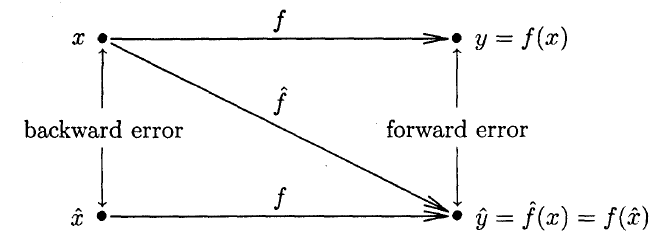
\includegraphics[width=0.5\textwidth]{schematic_diagram_of_forward_and_backward_error}
\end{wrapfigure}
\itmlthr{
	\item $x,f$:\@ exact input and func.\@
	\item $\hat{f}$:\@ approx.\@ func.\@
	\item $\hat{x}$:\@ exact val.\@ for $\hat{f}$ \\ \\ \\ \\ \\ \\ \\
}

\lvs
\itmltwo{
	\item $\hat{f}(x)=f(\hat{x})$ due to the choice of $\hat{x}$, which defines $\hat{x}$
	\item back.\@ err.\@ anly is easier, used to measure algo.\@ stability
	\item comp.\@ err.\@ $ \left\langle
		\begin{array}{lcl}
			\text{trunc.\@ err.\@} & : & \text{due to trunc.\@ of inf.\@ series, finite diff., \ldots} \\
			\text{round.\@ err.\@} & : & \text{due to finite-precs., rounding arith., \ldots}
		\end{array}
	\right.$
	\item $\tbf{total err.\@} = \hat{f}(\hat{x})-f(x) = \underbrace{\fbt{\hat{f}(\hat{x})-f(\hat{x})}}_{\text{comp.\@ err.\@}} + \underbrace{\big(f(\hat{x})-f(x)\big)}_{\text{data err.\@}}$
}

\tbl{Sensitivity}
$
	\left\{
	\begin{array}{lcl}
		\text{insensi./\trdbf{well-cond.}\@} & : & \text{input rel.\@ change} \leadsto \text{similiar rel.\@ change in sol.\@} \\
		\text{sensi./\trdbf{ill-cond.}\@} & : & \text{rel.\@ change in sol.\@ is much larger}\\
	\end{array}
	\right.
$

\tbl{Cond.\@ Num.\@}
\[
	\textrm{cond} = \dfrac{\fvt{\text{rel.\@ change in sol.\@}}}{\fvt{\text{rel.\@ change in input}}} =
	\dfrac{\big(f(\hat{x})-f(x)\big)/f(x)}{\fbt{\hat{x}-x}/x} =
	\dfrac{\fvt{\Delta y/y}}{\fvt{\Delta x/x}}
\]
\tvs
\itmltwo{
	\item $\textrm{cond} \geq 1\;(>10)$: sensi./ill-cond.\@ prob.\@
	\item $\fvt{\text{rel.\@ fore.\@ err.\@}} \lessapprox \textrm{cond} \cdot \fvt{\text{rel.\@ back.\@ err.\@}}$
	\itmind{\item[$\circ$] $\textrm{cond}$ $\Llr$ amplification factor}
	\itmind{\item[$\circ$] $\lessapprox$:\@ a rough est.\@ or \trdbf{upper bound} for the max.\@ cond.\@}
	\item $\textrm{cond} \approx \fvt{\dfrac{xf'(x)}{f(x)}} \; [\ref{eq:func_cond}]$
}

\pagebreak

\tbl{Stability}
$
	\left\{
	\begin{array}{ll}
		\underset{\text{(well-posed)}}{\text{math prob.\@}} &
		\left\langle
		\begin{array}{l}
			\text{sol.\@ exists, unique, depends continuously} \\
			\text{small input change } \slashed{\leadsto} \text{ abrupt change in sol.\@} \\
			\text{well-posed} \neq \text{sol.\@ is insensi.\@ to pertb.\@}
		\end{array}
		\right. \\
		\underset{\text{(stable)}}{\text{algo.\@ desp.\@}} &
		\left\langle
		\begin{array}{l}
			\text{rst.\@ rel.\@ insensi.\@ to pertb.\@ due to approx.\@} \\
			\text{rst.\@ is the exact sol.\@ to a \trdbf{nearby} prob.\@} \\
			\text{weaker:\@ \uwave{nearly} correct rst.\@ for \uwave{nearly} the correct prob.\@} \\
		\end{array}
		\right.
	\end{array}
	\right.
$

\tbl{Accuracy}
$
	\left\{
	\begin{array}{l}
		\text{closeness of comp.\@ sol.\@ to true sol.\@} \\
		\text{depends on algo.\@ cond.\@ and stability} \\
		\text{stability} \;\frdbs{\neq}\; \text{accuracy} \\
	\end{array}
	\right.
$
\begin{tabular}{c|c|c}
	~ & alog.\@ & prob.\@ \\
	\hline
	\multirow{2}{*}{inaccuracy} & stable & ill-cond.\@ \\
	& unstable & well-cond.\@ \\
	\hline
	accuracy & stable & well-cond.\@ \\
\end{tabular}

\tbl{Mach.\@ Precs.\@}
$
	\left\{
	\begin{array}{l}
		\vep_m = \arg\min_\vep \textrm{fl}(1+\vep)>1 \\
		\fvt{\dfrac{\textrm{fl}(x)-x}{x}} \leq \vep_m \\
	\end{array}
	\right.
$
\itmltwo{
	\item $\textrm{fl}(x)$:\@ round to nearest, $\textrm{fl}(x \oplus y)=(x \oplus y)(1+\delta) \esp \fvt{\delta} \leq \vep_m$
	\item $\vep_m$ determines the \uwave{max.\@ rel.\@ err.\@} in representing a real num.\@ $x$
}

\begin{center}
\begin{tabular}{|c|c|c|c|}
	\cline{1-4}
	\multirow{3}{*}{~} & \multicolumn{3}{c|}{\trdbf{Total Err.}\@} \\ \cline{2-4}
	~ & \multicolumn{2}{c|}{comp.\@ err.\@} & \multirow{2}{*}{data err.\@} \\ \cline{2-3}
	~ & trunc.\@ err.\@ & round.\@ err.\@ & ~ \\ \cline{1-4}
	\multirow{2}{*}{howto est.\@} & \multirow{2}{*}{theoretical anly.\@} & back.\@ err.\@ anly.\@ & \multirow{2}{*}{cond.ing,\@ \uwave{$\textrm{cond}$}} \\
	~ & ~ & hard to quantify & ~ \\ \cline{1-4}
	\multirow{2}{*}{howto rdc.\@} & \multirow{2}{*}{aglo.\@ selction} & \trdbf{stable} algo.\@ & change prob.\@ form.\@ \\
	~ & ~ & tips{$^\dagger$}, dbl-precs.\@ & improve cond.ing \\ \cline{1-4}

\end{tabular}
\end{center}
\itmltwo{
	\item avoid \uwave{subtractive cancellation} in nums.\@ of nearly equal mag.\@
	\item avoid adding \uwave{large and small} nums.\@
	\item adjust the \uwave{order} of additions
}

\tbl{Mat.\@ Cond.\@}
\mvs{1em}
\[
	\kappa(\fbs{A}) \triangleq \fVt{\fbs{A}} \cdot \fnVt{\fbs{A}^{-1}}
\]
\tvs
\itmltwo{
	\item $\kappa$ is def.\@ for \uwave{sqr.\@ non-singlr.\@ mat.}, $\kappa(\fbs{A})=\infty$ if $\fbs{A}$ singlr.\@
	\item $\kappa(\fbs{A}) \geq 1$, $\kappa(\fbs{I})=1$, $\kappa(\gamma\fbs{A})=\kappa(\fbs{A})$, $\kappa(\fbs{D})=\fbt{\max\fvt{d_i}}\big/\fbt{\min\fvt{d_i}},\fbs{D}=\textrm{diag}(d_i)$
}
\begin{figure}[h]
	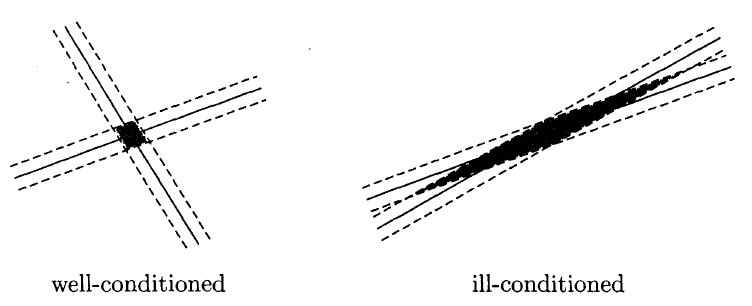
\includegraphics[width=0.5\textwidth]{well_conditioned_and_ill_conditioned_linear_system}
	\centering
\end{figure}

\tbl{Err.\@ Bounds}
\mvs{1em}
\[
	\dfrac{\fVt{\Delta\fbs{x}}}{\fVt{\fbs{x}}} \lessapprox \kappa_1(\fbs{A}) \dfrac{\fVt{\Delta\fbs{b}}}{\fVt{\fbs{b}}} \;[\ref{eq:b_perb_cond}] \qsp
	\dfrac{\fVt{\Delta\fbs{x}}}{\fVt{\hat{\fbs{x}}}} \lessapprox \kappa_2(\fbs{A}) \dfrac{\fVt{\fbs{E}}}{\fVt{\fbs{A}}} \;[\ref{eq:A_perb_cond}] \qsp
	\dfrac{\fVt{\Delta\fbs{x}}}{\fVt{\fbs{x}}} \lessapprox \kappa_3(\fbs{A}) \fbt{\dfrac{\fVt{\Delta\fbs{b}}}{\fVt{\fbs{b}}} + \dfrac{\fVt{\fbs{E}}}{\fVt{\fbs{A}}}} \;[\ref{eq:Ab_perb_cond}]
\]
\tvs
\itmltwo{
	\item $\frdbs{\lessapprox}$:\@ approx.\@ bounded by
	\item $\kappa$ provides a quantitative bound for the err.\@ in comp.\@ sol.\@
	\item $\kappa_1$ bounds the \uwave{max.\@ rel.\@ change in sol.}\@ due to a given rel.\@ change \uwave{in vec.\@ $\fbs{b}$}
	\item similar rst.\@ $\kappa_2$ holds for rel.\@ change \uwave{in mat.\@ $\fbs{A}$}
	\item mat.\@ scaling affects $\kappa$ rather than the singlr.\@
	\item $\dfrac{\fVt{\hat{\fbs{x}}-\fbs{x}}}{\fVt{\fbs{x}}} \lessapprox \kappa(\fbs{A})\vep_m$ if input data accurate to mach.\@ precs.\@
}

\tbl{Residual}
$
	\left\{
	\begin{array}{l}
		\fbs{r} = \fbs{b} - \fbs{A}\hat{\fbs{x}} \text{ where } \hat{\fbs{x}} \text{ is approx.\@ sol.\@} \\
		\text{rel.\@ res.\@} \;\frdbs{\triangleq}\; \dfrac{\fVt{\fbs{r}}}{\fVt{\fbs{A}} \cdot \fVt{\hat{\fbs{x}}}}
	\end{array}
	\right.
$
\[
	\dfrac{\fVt{\Delta\fbs{x}}}{\fVt{\hat{\fbs{x}}}} \leq \kappa(\fbs{A}) \dfrac{\fVt{\fbs{r}}}{\fVt{\fbs{A}} \cdot \fVt{\hat{\fbs{x}}}} \;[\ref{eq:rel_res_cond}]
\]
\tvs
\itmltwo{
	\item \uwave{size of res.\@} is considered rel.\@ to the size of prob.\@ and sol.\@
	\item small rel.\@ res.\@ $\leadsto$ small rel.\@ err.\@ \ifof $\fbs{A}$ is well-cond.\@
	\item large rel.\@ res.\@ $\leadsto$ large back.\@ err.\@ in mat.\@ $\leadsto$ unstable algo.\@ $[\ref{eq:A_perb_rel_res}]$
	\item stable algo.\@ $\Llr$ small rel.\@ res.\@ (irresp.\@ to cond.ing)
}
